\section{Discrete Kalman filter}
This section explains our method for constructing a discrete Kalman filter for our cargo-ship to estimate a rudder-bias and filter out high-frequency wave-influences, and compares the system response with the Kalman filter to that of the system used in \cref{sec:Autopilot}.


\subsection{Problem a}
To implement a discrete Kalman filter we naturally need a discrete state-space representation of our cargo-ship dynamics. The code needed to perform this discretization with a sample frequency of $10 \textrm{ Hz} \rightarrow (T_s = 0.1\textrm{ s})$ is found in \cref{fig:p5p5_init} and in parts of \cref{fig:p5p5c_model}. We use the built-in functionality in MATLAB to get our discrete system-matrices.


\begin{equation}\label{eq:sys_discrete}
\begin{aligned}
    \mathbf{A_d} &= 
    \begin{bmatrix} 
    0.9970 & 0.0992 & 0 & 0 & 0 \\
    -0.0607 & 0.9835 & 0 & 0 & 0 \\
    0 & 0 & 1 & 0.0999 & -1.0763\cdot10^{-5} \\
    0 & 0 & 0 & 0.9986 & -2.1520\cdot10^{-4} \\
    0 & 0 & 0 & 0 & 1
    \end{bmatrix}, 
    \quad
    \mathbf{B_d} =
    \begin{bmatrix} 
    0 \\
    0 \\
    1.073\cdot10^{-5} \\
    2.1520\cdot10^{-4} \\
    0 
    \end{bmatrix} 
    \\
    \mathbf{C_d} &= \begin{bmatrix} 
    0 & 1 & 1 & 0 & 0
    \end{bmatrix}, 
\end{aligned}
\end{equation}

Note that the system matrix $\mathbf{E}$ isn't discretized in our code, neither is it listed here as one of the discrete system matrices since it's only purpose is to discretize $\mathbf{Q}$, and we used van Loan's method to do this, which makes it unnecessary to find $\mathbf{E_d}$. \cite{kalman}

\subsection{Problem b}

To find the variance of the measurement noise we ran a simulation with $0^{\circ}$ as rudder input so our output would be purely the measurement noise, $v$. We then extracted the data as a time series and used the Matlab function \texttt{var(v)}.

The result gave us the $\mathbf{R}$ for our system, $\mathbf{R} = 0.0020$.


\subsection{Problem c}

In order to construct a Kalman filter for our system we need a complete discretized model, and so we were provided with the matrices in \cref{eq:p5p5c_given}.

\begin{equation} \label{eq:p5p5c_given}
\begin{aligned}
    \mathbf{w} &= 
    \begin{bmatrix} w_w & w_b \end{bmatrix}, 
    \quad
    E\{\mathbf{ww}^T\} = \mathbf{Q} = 
    \begin{bmatrix}
        30 & 0 \\
        0  & 10^{-6}
    \end{bmatrix},
    \\
    \mathbf{P}_0^- &= 
    \begin{bmatrix} 
    1 &   0   &   0   & 0 &  0 \\
    0 & 0.013 &   0   & 0 &  0 \\
    0 &   0   & \pi^2 & 0 &  0 \\
    0 &   0   &   0   & 1 &  0 \\
    0 &   0   &   0   & 0 & 2.5 \cdot 10^{-4}
    \end{bmatrix}, 
    \mathbf{\hat{x}}_0^- = 
    \begin{bmatrix} 
    0 \\
    0 \\
    0 \\
    0 \\
    0 
    \end{bmatrix}
\end{aligned}
\end{equation}

From these given matrices, our discretized system-matrices and the measurement noise variance, $\mathbf{R}$ we have everything needed to construct our discrete Kalman filter. We start by discretizing the disturbance variance matrix $\mathbf{Q}$ using van Loan's method\cite{kalman} and the measurement noise variance matrix $\mathbf{R}$, the result is seen in \cref{eq:discrete_variances}, where $\mathbf{Q_d}$ denotes the discretized disturbance variance matrix and $\mathbf{R_d}$ denotes the discretized noise variance.

\begin{equation}\label{eq:discrete_variances}
\begin{aligned}
    \mathbf{Q_d}&=
    \begin{bmatrix}
        2.6889\cdot10^{-7} & 4.0165\cdot10^{-6} & 0 & 0 & 0 \\
        4.0165\cdot10^{-6} & 8.0331\cdot10^{-5} & 0 & 0 & 0 \\
        0 & 0 & 2.3170\cdot10^{-18} & 5.7917\cdot10^{-17} & -3.5879\cdot10^{-13} \\
        0 & 0 & 5.7917\cdot10^{-17} & 1.5443\cdot10^{-15} & -1.0763\cdot10^{-11} \\
        0 & 0 & -3.5879\cdot10^{-13} & -1.0763\cdot10^{-11} & 1.000\cdot10^{-7}
    \end{bmatrix}
    \\
    \mathbf{R_d}&= \frac{\mathbf{R}}{T_s}= 0.0199
\end{aligned}
\end{equation}

To implement our discrete controller in simulink we use code from \cref{fig:p5p5c} to construct a data-struct which is in turn  sent over to the Kalman filter "fcn-block" in Simulink. Simulink model \cref{fig:p5p5c_model} shows the implementation of the Kalman filter.

The algorithm to perform the discrete Kalman filtering is explained in \cite{kalman}, and our implementation of this algorithm is found in \cref{fig:kalman_filter}. As proven in lecture and in \cite{kalman}, the Kalman filter will make the optimal choice between measurement and estimate at each iteration of the algorithm, and perform a blending of the two signals to compute its desired output. In essence it reduces the variance of its output compared to its input. In our case we feed it our measurement of $\psi$, apply the Kalman filter, and get a wave-filtered $\psi$ with a lower variance.

\Cref{fig:p5p5c_Kalman_values} shows the outputs of the Kalman filter, $\psi_{filtered}$ and $b$. These values are obtained by running a simulation without disturbances (only measurement noise) with the model mentioned above, so the Kalman filter takes in the input $u$ and the measurement $y$, but the output of the filter doesn't enter the closed loop system.


\begin{figure}[h]
	\centering
	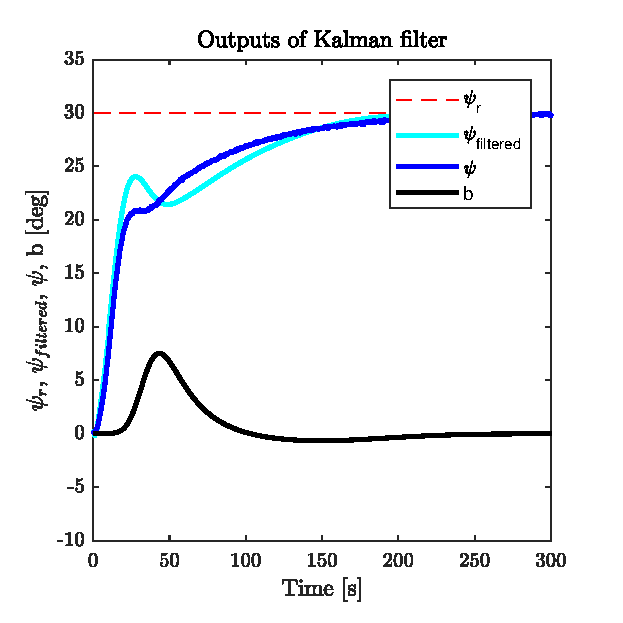
\includegraphics[width=\textwidth]{figures/p5p5c.eps}
	\caption{Estimated values form the Kalman filter}
\label{fig:p5p5c_Kalman_values}
\end{figure}

\subsection{Problem d}

The first step to adding the output of the Kalman filter to our closed loop system was to add estimated rudder bias, $b$, as a feed forward to the closed loop as shown in \cref{fig:p5p5d_model} in \cref{sec:simulink}. With this model we ran a simulation with current disturbance and no wave disturbance. The resulting response is shown in \cref{fig:p5p5d_current_disturbance}. If compared to the response from \cref{sec:Autopilot_c}, shown in \cref{fig:p5p3c_current_distur} we see that the stationary error is no longer present in the heading, meaning the Kalman filter would have made the addition of an I-term in the controller obsolete.

\begin{figure}[h]
	\centering
	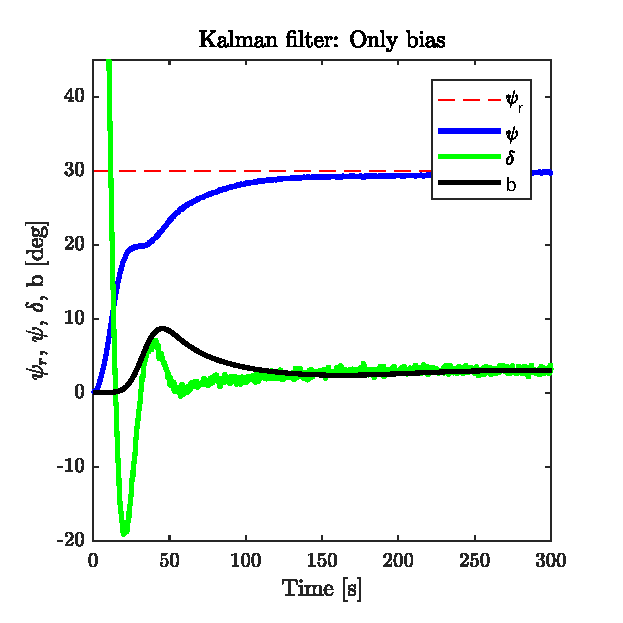
\includegraphics[width=\textwidth]{figures/p5p5d.eps}
	\caption{System response with feed forward from estimated bias}
\label{fig:p5p5d_current_disturbance}
\end{figure}


\subsection{Problem e}

By changing the feedback loop from the measured heading to the wave-filtered heading from the Kalman filter we aim to further improve our system. We simulate the system with both current and wave disturbance turned on to get the result shown in \cref{fig:p5p5e_system_response}. We compare this response to the one in \cref{fig:p5p3d_wave_distur} from \cref{sec:Autopilot_d} and see there's been a dramatic reduction in the magnitude of the high frequency rudder response, $\delta$. The system is no longer trying as hard to correct deviations from the course set-point caused by the waves because the Kalman filter is smoothing out the signal fed back as the process value. Limiting this high-frequency rudder-input makes it much easier on the actuator for the rudder, reducing the wear and tear on it. The Kalman filter has now addressed the most prominent issues with both the sources of disturbance applied to the system without having to implement any of the changes proposed in \cref{sec:Autopilot_eval}

\begin{figure}[h]
	\centering
	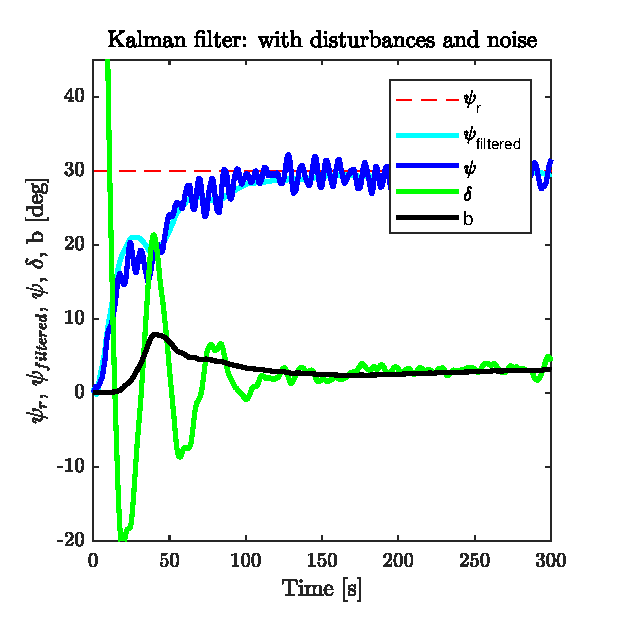
\includegraphics[width=\textwidth]{figures/p5p5e.eps}
	\caption{System response and filter values with feed forward and filtered feedback loop}
\label{fig:p5p5e_system_response}
\end{figure}


To smooth out the measured heading the Kalman filter has to estimate the influence the wave disturbance has on it and counteract it. In \cref{fig:p5p5e_wave_influence} we compare the actual wave influence on the system to what the Kalman filter estimates it to be. We see that it's a near match, but the filter falls short in the peaks of the wave signal. The estimation of $\psi_w$ is good, but not perfect so there is room for improvement on our Kalman filter. Right now we update our Kalman filter with the same frequency as the wave-signal it is trying to estimate. By increasing the frequency we run our Kalman algorithm with we might get better results as this will cause us to get more estimates per period of the wave signal. However, the trade-off here is that running the Kalman filter seems to be quite computationally heavy already, meaning that any actual implementation on a real cargo-ship would require some serious computing power. Even though we do not have a perfect match on our $\psi_w$ estimate we note that our autopilot performs quite well.


\begin{figure}[h]
	\centering
	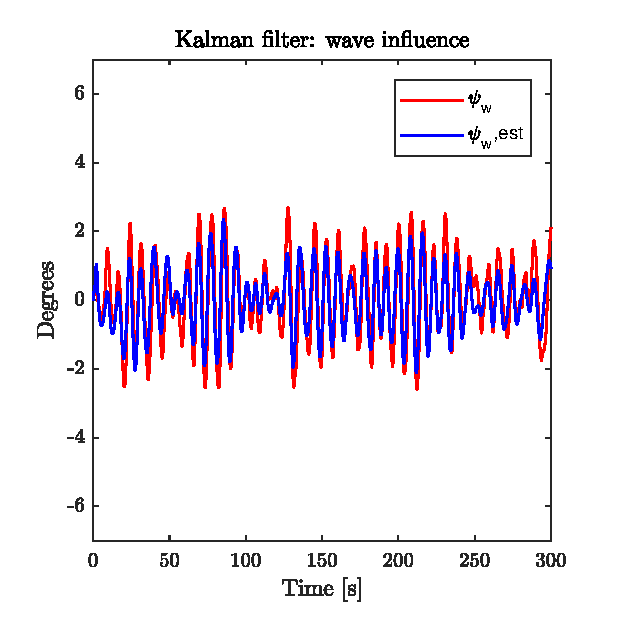
\includegraphics[width=\textwidth]{figures/p5p5e_wave_influence.eps}
	\caption{Wave influence and estimated wave influence}
\label{fig:p5p5e_wave_influence}
\end{figure}